\chapter{Seitenkanalangriffe}
\label{sec:seitenkanalangriffe}
Lange wurden in der Kryptographie die einzelnen Komponenten als Black
Box betrachtet. Man ist davon ausgegangen, dass eine solche Komponente
lediglich definierte Eingaben, wie z.B. Klartext und Schlüssel, bekommt,
um daraus eine definierte Ausgabe zu berechnen. Praktisch kommen jedoch
weitere Eingaben (Strom), weitere Ausgaben (elektromagnetische
Abstrahlung) sowie interne Zustände (und dadurch andere Laufzeiten)
hinzu, die einem Angreifer Informationen über das Geheimnis der
Komponente liefern können. Es gibt eine ganze Reihe solcher
\emph{Seitenkanäle}, die Informationen nach außen tragen
können. Beispiele hierfür sind:
\begin{itemize}
\item Stromverbrauch
\item Laufzeiten
\item Elektromagnetische Abstrahlung
\item Akkustische Abstrahlung
\end{itemize}

Die Erkenntnis, dass solche Phänomene geeignet sind, Geheimnsse einer
Implementierung von kryptographischen Verfahren preis zu geben, ohne
dass das Verfahren an sich unsicher ist, hat seit der Mitte der 1990er
Jahren zu einer intensiven Beschäftigung mit diesem Problem geführt. 

In diesem Kapitel werden einige grundlegende Angriffe und Gegenmaßnahmen
für Seitenkanalangriffe dargestellt.

\section{Simple Power Analysis}
\label{sec:simple-power-analys}
Ein einfacher Seitenkanalangriff ist die \emph{Simple Power
  Analysis(SPA)}. Dabei wird der Stromverbrauch einer CPU gemessen,
während diese einen Algorithmus ausführt. Als Beispiel wird im folgenden
untersucht, wie mittels einer SPA der geheime Schlüssel bei einer naiven
RSA-Implementierung gefunden werden kann.
\subsection{SPA der RSA-Entschlüsselung}
Wird ein RSA-Chiffrat entschlüsselt, so berechnet wird \[\plaint
  =\ciphert^d \mod N\] berechnet. Eine gängige Implementierung ist das
Square-and-Multiply-Verfahren in Algorithmus \ref{alg:Square-and-Multiply}. 
\begin{algorithm}[!h]
\caption{Square-and-Multiply-Verfahren}
\label{alg:Square-and-Multiply}
\begin{algorithmic}
\Procedure{SaM}{$x, b$}\Comment{Berechnet $x^k \mod N$, wobei $b$ die
  Binärdarstellung von $k$ ist}

  \State $x \gets C$
  \State $z \gets 1$
  \For{$i\text{ in }\{0, \dots, n-1\}$}
    \If{$b[i]==1$}
      \State $z \gets z \cdot x \mod N$
    \EndIf
    \State $x \gets x^2 \mod N$
  \EndFor
  \State \textbf{return} $z$
\EndProcedure
\end{algorithmic}
\end{algorithm}

Hierbei wird $d$ bitweise abgearbeitet. Je nach dem, ob das $i$-te Bit
von $d$ $1$ oder $0$ ist, werden eine oder zwei Multiplikationen
durchgeführt. Ergibt eine Messung des Stromverbrauchs also Einen Verlauf
wie in Abb. \ref{abb:power-attack}, so lässt sich daraus schließen, dass
dort erst eine $0$ und anschließend eine $1$ im Schlüssel verarbeitet wurden.

\begin{figure}[h]
  \centering
  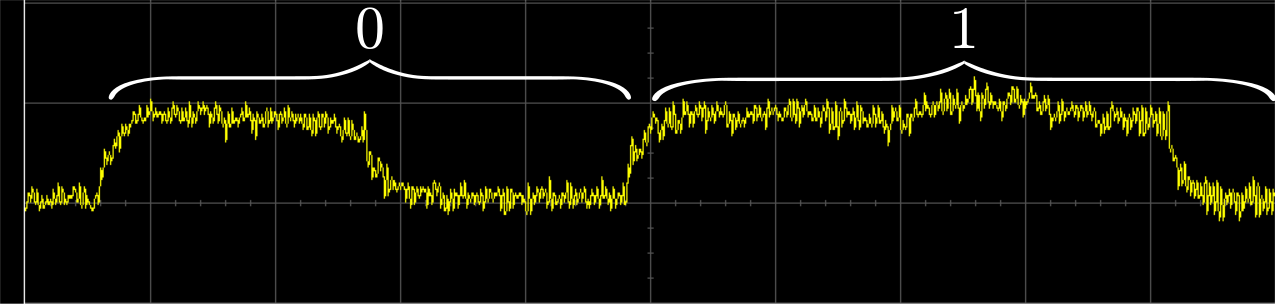
\includegraphics[width=\textwidth]{images/Power_attack}
  \caption{Messung des Stromverbrauchs für SPAs}
  \label{abb:power-attack}
\end{figure}

\subsection{Gegenmaßnahmen}
Um SPAs zu vermeiden, bieten sich Gegenmaßnahmen auf Hardware- und
Algorithmusseite an. Hardwareseitig kann man den Stromverbrauch
unabhängig von den ausgeführten Opereationen konstant halten. Zudem kann
man die Algorithmen so implementieren, dass ein keine bedingten Sprünge
in Abhängigkeit vom Geheimnis gibt. Außerdem können Dummy-Berechnungen
genutzt werden, um den Stromverbrauch und die Laufzeit  zu verrauschen.

\section{Differential Power Analysis (DPA)}
Eine aufwändigere, aber mächtigere Technik, um aus Power-Traces
Informationen über einen geheimen Schlüssel zu gewinnen, ist die
\emph{Differential Power Analysis (DPA)}. Um eine DPA durchführen zu
können, muss der Angreifer die Implementierung des Algorithmus kennen,
der auf dem Prozessor läuft. Auserdem braucht er eine möglichst große
Menge an Trace-Message-Paaren $(T_X, X)$, also jeweils den Stromverbrauch bei der
Entschlüsselung einer gegeben Nachricht (oder eines gegebenen
Chiffrats).
Ein Angreifer rät nun einen Teil $s$ des Geheimnis $S$. Dann simuliert
er den Algorithmus für alle $X$ und sortiert die Eingaben in zwei
Gruppen \calL, \calH, wobei
\begin{eqnarray*}
\calL & := &\{X| \texttt{Simulation mit $X$ hat einen niedrigen
  Stromverbrauch}\},\\
\calH & := &\{X| \texttt{Simulation mit $X$ hat einen hohen
  Stromverbrauch}\}.
\end{eqnarray*}
Anschließend betrachtet der Angreifer den durchschnittlichen
\textit{realen} Stromverbrauch beider Gruppen. War $s$ richtig geraten,
so sollte sich der reale Durschnittsverbrauch beider Gruppen stark
unterscheiden. Tut er dies nicht, so war $s$ wohl falsch geraten.

\subsection{Gegenmaßnahmen}
Um sich von DPAs zu schützen, kann man versuchen, den Stromverbrauch
durch zusätzliche Berechnungen zu verrauschen. Beispielsweise kann eine
Entschlüsselung vorgenommen werden mit $\plaint = \C^d = \frac{(R\cdot
  C)^d}{R^d}$, wobei $R$ zufällig gewählt wird.

\section{Cold Boot Attacks}
\emph{Cold Boot Attacks} machen es sich zunutze, dass der Hauptspeicher
Informationen erst langsam verliert, wenn die Stromversorgung
unterbrochen wird. Die Zeit, die es braucht, bis die Daten verloren
sind, lässt sich beträchtlich hinauszögern, wenn der Speicher (z.B. mit
flüssigem Stickstoff) heruntergekühlt wird. Damit kann der Zeitraum für
einen Angriff von einigen Sekunden auf mehrere Stunden gestreckt werden
\cite{Halderman08leastwe}.

Setzt ein System eine Festplattenverschlüsselung ein, so muss der
Schlüssel im Speicher gehalten werden, da der Benutzer nicht bei jedem
Fesplattenzugriff nach dem Schlüssel gefragt werden kann. Wenn ein
Angreifer jetzt das System im laufenden Betrieb in seinen Besitz bringt,
kann er den Hauptspeicher herunterkühlen und den Strom abstellen, ohne
das System herunterzufahren. So hat das Betriebssystem nicht die
Möglichkeit, die entsprechenden Speicherbereiche zu überschreiben. Jetzt
kann der Angreifer auf dem Hauptspeicher ein minimales System starten,
dass möglichst wenig Speicher braucht. Dieses minimale System hat die
Möglichkeit, die Speicherbereiche auszulesen, in denen der Schlüssel
gespeichert war. Damit kann der Angreifer dann die Festplatte
entschlüsseln.

\subsection{Gegenmaßnahmen}
Gegen Cold Boot Attacks gibt es Ansätze auf verschiedenen Ebenen. Auf
Ebene des BIOS gibt es die Möglichkeit, dass das Bios bei jedem Start
den Hauptspeicher neu initialisiert und dabei bestehende Daten
löscht. Damit ist sichergestellt, dass eine Cold Boot Attack nicht vom
eigenen Rechner stattfindet.

Eine weitere Möglichkeit besteht darin, den Schlüssel nicht im
Hauptspeicher, sondern im Prozessor-Cache zu speichern. Der Cache ist,
im Gegensatz zum Hauptspeicher, nicht einzelnt entnehmbar und durchläuft
beim Start des Prozessors eine Initialisierung, die die Inhalte des
Caches überschreibt. Dieser Ansatz führt jedoch zu massiven
Leistungseinbußen, da große Teile des Caches für andere Informationen
nicht mehr zur Verfügung stehen.
\section{Theoretische Modelle}
Viele Gegenmaßnahmen gegen Seitenkanalangriffe sind \glqq
Ad-hock\grqq-Ansätze, die nicht auf formalen Methoden
basieren. Wünschenswert sind aber Systeme, deren Sicherheit beweisbar
ist. Dafür möchte man die Eigenschaft eines Systems, sicher gegenüber
Seitenkanalangriffen zu sein, in einem formalen Modell darstellen
können. Solche Modelle sind Gegenstand aktueller Forschung. Theoretische
Modelle gegen solche Seitenkanalangriffe werden hier nur oberflächlich
behandelt. Als Einstieg für eine tiefere Beschäftigung mit dem Thema
bietet sich \cite{mol2010} an.

Um Seitenkanäle zu beschreiben, verwendet man beispielsweise eine
\emph{Leakage}-Funktion. Eine solche Funktion beschreibt, welche
Informationen eine Implementierung nach außen gibt. Die Ausgabe hängt ab
vom internen Zustand $S$, einer Eingabe $Y$ sowie einem zufälligen
Rauschen $R$. Darauf aufbauend werden dann verschiedene Arten von
Angriffen unterschieden. 
\subsection{Unbounded (continuous) computational-leakage}
Hierbei werden Informationen durch Prozessoroperationen nach Außen
getragen. Dabei geht man davon aus, dass nur Informationen, die im
Prozessor verarbeitet werden, von außen gelesen werden können. Solche
Angriffe sind die oben beschriebenen Techniken SPA und DPA.

Es wird davon ausgegangen, dass der Algorithmus, der auf der Hardware
läuft, rundenbasiert berechnet wird. Modelliert wird ein Angriff
dadurch, dass sich der Angreifer vor der $i$-ten Runde eine
Leakage-Funktion $f_i$ wählt und nach der $i$-ten Runde $f_i(S_{i-1})$
erhält, wobei $S_{i-1}$ der interne Zustand der Komponente zum
Zeitpunkt $i-1$ ist. Der Angreifer soll für eine beliebige, polynomiell
beschränke Funktion $f_i$ das Geheimnis nicht lernen.
\subsection{Memory-Leakage Attacks}
Mit dem oben beschriebenen Modell wird eine wichtige Klasse von
Seitenkanalangriffen nicht modelliert. Cold Boot Attacks können
beispielsweise Informationen leaken, die nicht im Prozessor verarbeitet
wurden. Solche und ähnliche Angriffe modelliert man dadurch, dass der
Angreifer eine Funktion $f$ wählt. Er erhält dann $f(S)$, wobei $S$ der
geheime Zustand ist. $f$ hat hierbei einen \emph{Leakage-Parameter} $l$
als obere Schranke, und es gilt, dass $|l|<|S|$, also dass die Funktion
nicht den gesammten geheimen Zustand aufdeckt. Ein System ist sicher
gegen Memory-Leakage Attacks, wenn der Anfgreifer für beliegige solche
Funktionen nicht an den geheimen Zustand kommt.

\section{Fazit}
Seitenkanalangriffe sind eine wichtige Klasse von Angriffen gegen
Implementierung von kryptographischen Komponenten. Sie sind aber nur
schwer mit formalen Methoden in den Griff zu bekommen. Insbesondere
erfordern sie andere Vorgehensweisen, als sie in anderen, eher formal
geprägten Bereichen der Kryptographie üblich sind. Sie zu analysieren
erfordert Kenntnisse in den theoretischen Aspekten von Kryptographie, in
der Implementierung von kryptographischen Komponenten sowie in den
Eigenschaften der Hardware, auf denen die Komponenten eingesetzt
werden. 